\documentclass[a4paper,11pt]{jsarticle}

% 数式
\usepackage{amsmath,amsfonts}
\usepackage{amsthm}
\usepackage{bm}
\usepackage{mathtools}
\usepackage{amssymb}

% 表
\usepackage[utf8]{inputenc}
\usepackage{diagbox} % 斜線付きセルを作成するために必要
\usepackage{booktabs} % 表の罫線を美しくするために必要
\usepackage{hhline} % 水平罫線を制御するために必要

% 画像
\usepackage[dvipdfmx]{graphicx}
\usepackage{ascmac}
\usepackage{physics}
\usepackage{float} % 追加

% 図
\usepackage[dvipdfmx]{graphicx}
\usepackage{tikz} %図を描く
\usetikzlibrary{positioning, intersections, calc, arrows.meta,math} %tikzのlibrary

% ハイパーリンク
\usepackage[dvipdfm,
  colorlinks=false,
  bookmarks=true,
  bookmarksnumbered=false,
  pdfborder={0 0 0},
  bookmarkstype=toc]{hyperref}

% 式番号を章ごとにリセット
\numberwithin{equation}{section}

\begin{document}

\title{B4ゼミ\#3}
\author{大上由人}
\date{\today}
\maketitle

\setcounter{section}{2}
\section{確率熱力学}
\subsection{Shanonエントロピー}
\subsubsection{Stochastic エントロピー}
\begin{itembox}[l]{\textbf{Def.Stochastic エントロピー}}
    M個の事象$\{x_1, x_2, \cdots, x_M\}$があるとき、事象$x_i$が起こる確率を$p_i$とする。このとき、事象$x_i$の確率的エントロピーは、
    \begin{align}
        s(x_i) = -\ln p_i
    \end{align}
    と定義される。
\end{itembox}
この量は、surprisalとも呼ばれ、ある事象がどれほど"驚くべき事象か"を表している。
例えば、$p_i = 1$のとき、$s(x_i) = 0$であるが、これは、事象$x_i$が起こることが確定しているので、"驚くべき事象"ではないことがわかる。
逆に、非常に確率が小さい事象$x_i$が起こるとき、$s(x_i)$は非常に大きな値をとる。これは、事象$x_i$が起こることは非常に驚くべき事象であることを表している。

Stochasticエントロピーは、以下の要素を満たす。
\begin{itemize}
    \item 確率分布$p_i$について連続関数である。
    \item 独立な分布$(p,p')$に対して、$s(p_p') = s(p) + s(p')$が成立する。
\end{itemize}
実は、この2つの条件を満たす関数は、$s(p) = -\ln p + C$の形のみであることが示される。

\begin{itembox}[l]{\textbf{Thm.}}
    $f(p)$が、以下の性質を持つとき、その関数形は定数項を除いて、$-\ln p$の形に一意に決まる。
    \begin{itemize}
        \item $f(p)$は、確率分布$p$に対して連続関数である。
        \item $f(p)$は、独立な分布$(p,p')$に対して、$f(p_p') = f(p) + f(p')$が成立する。
    \end{itemize}
\end{itembox}
\textbf{Prf.}\\
\indent
$a^{n/m} = b \; (n, m \in \mathbb{N}, m \neq 0, a, b \in \mathbb{R})$とする。
\begin{alignat*}{4}
  f(a) &= f(a^{1/m} \cdot a^{1/m} \cdots a^{1/m}) \\
  &= m f(a^{1/m}) && \quad (\text{加法性}) \\
  f(b) &= f(a^{n/m}) && \quad (\text{$b$の定義}) \\
  &= n f(a^{1/m}) && \quad (\text{加法性})
\end{alignat*}
$f(a^{1/m})$を消去すると、$f(b)=\frac{n}{m} \cdot f(a)$となる。\\
$a$をNapier数とし、$b=x(>0)$とおくと、$\forall x \in \{ x \mid \ln{x} \in \mathbb{Q} \}$に対して
\begin{align}
  f(x) = f(\mathrm{e}) \ln{x}
\end{align}
が成り立つ。
有理数の集合が実数内で稠密であることと関数$f$の連続性から、\\
$f(x) \propto - \ln{x} \; (x \geq 0)$となる。
TODO精査
\qed\\

\subsubsection{Shanonエントロピー}
Stochasticエントロピーの平均として、Shanonエントロピーが定義される。

\begin{itembox}[l]{\textbf{Def.Shanonエントロピー}}
    $M$個の事象$\{x_1, x_2, \cdots, x_M\}$があるとき、事象$x_i$が起こる確率を$p_i$とする。このとき、確率変数$x$のShanonエントロピーは、
    \begin{align}
        H(x) = -\sum_{j} p_j \ln p_j
    \end{align}
    と定義される。
\end{itembox}
エントロピーは、事象の不確定性を表す量であるといえる。例えば、二項分布のエントロピーをグラフにすると、以下のようになる。
\begin{figure}[H]
    \begin{center}
    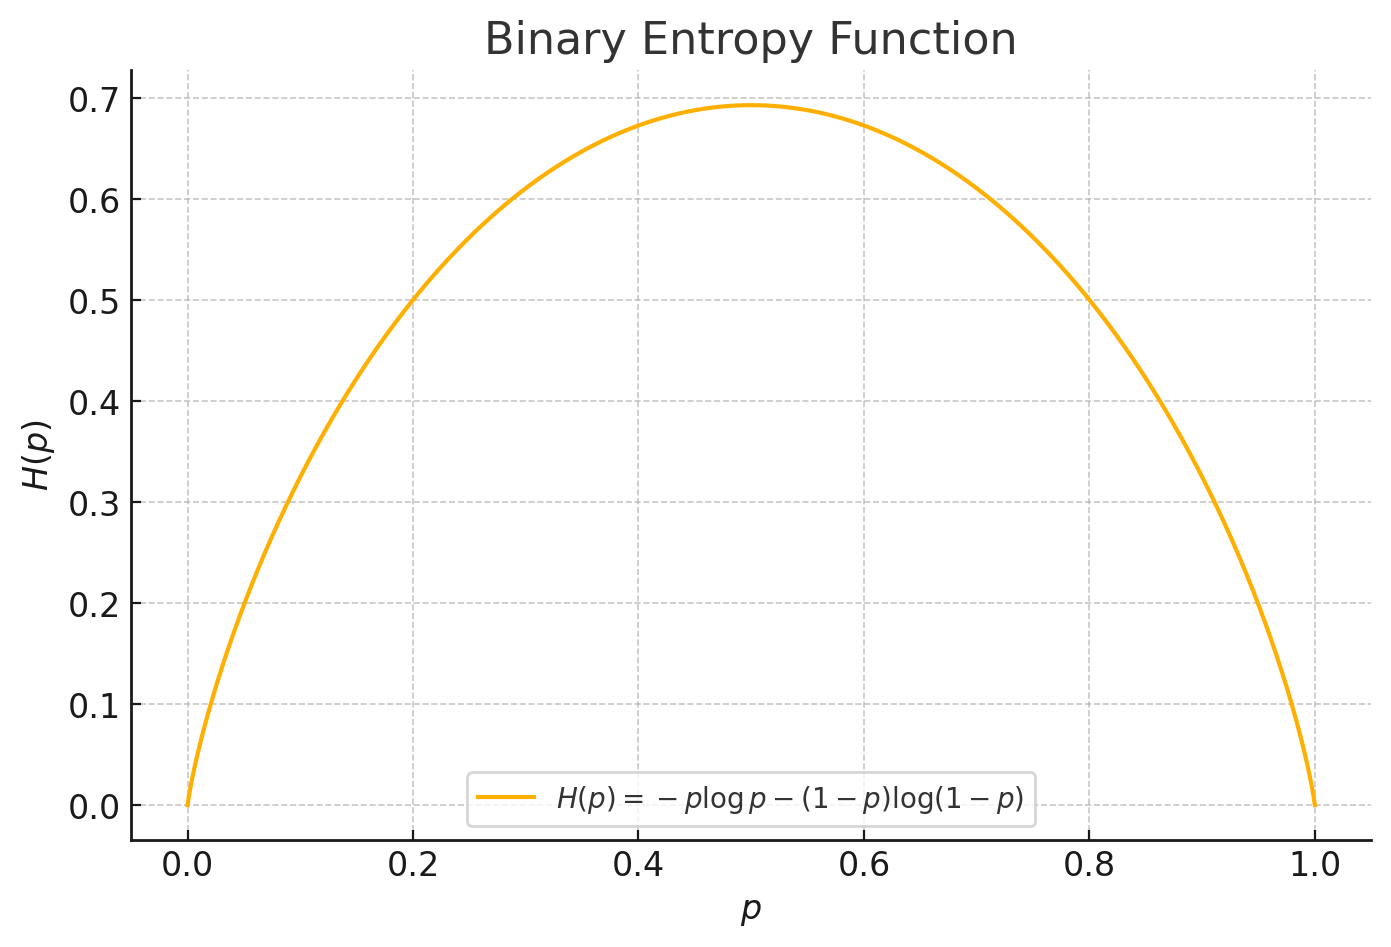
\includegraphics[width=100mm]{entropy.png}
    \end{center}
    \caption{二項分布のエントロピー}
    \label{fig:entropy}
\end{figure}
\indent
このとき、$p=\frac{1}{2}$のとき、エントロピーは最大値をとる。例えば、これをコイン投げに例えると、$p=\frac{1}{2}$のとき、表と裏が均等に出るので、コインを投げる前に、表が出るか裏が出るかは全くわからない。
しかし、$p\neq \frac{1}{2}$のとき、コインの出方が偏っているということになり、ある程度どちらが出るか予測できる。とくに、$p=0$または$p=1$のとき、エントロピーは0となるが、これは、事象の不確実性が0であることを表している。
また、一般のn変数の確率分布に対しても、分布が一様分布であるとき、エントロピーは最大値をとることが知られている。\footnote{
    Lagrangeの未定乗数法を用いればすぐに確かめられる。
}

これまでは、どのような事象が起こりそうかまったくわからない状況を取り扱っていたが、ある程度その情報がわかっていることもある。
このような場合は、不確実性を、条件付きShanonエントロピーによって表すことができる。
\begin{itembox}[l]{\textbf{Def.条件付きShanonエントロピー}}
    事象$y$のもとでの事象$x$のShanonエントロピーは、
    \begin{align}
        H(x|y) &= -\sum_{i,j}P(x_i,y_j) \ln P(x_i|y_j)\\
        &= -\sum_{j}P(y_j) \sum_{i}P(x_i|y_j) \ln P(x_i|y_j)
    \end{align}
    と定義される。
    ただし、$P(x_i,y_j)$は、事象$x_i$と$y_j$の同時分布である。
\end{itembox}
特徴をつかむために、コイントスの例を再び考えてみる。

\begin{table}[H]
    \centering
    \caption{コインの確率分布}
    \label{tab:coin}
    \begin{tabular}{cccc}
        \toprule
        & 表(Heads) & 裏(Tails) & 使用確率 \\
        \midrule
        コイン A & $\frac{1}{3}$ & $\frac{2}{3}$ & $\frac{1}{5}$ \\
        コイン B & $\frac{2}{3}$ & $\frac{1}{3}$ & $\frac{1}{5}$ \\
        コイン C & $\frac{1}{2}$ & $\frac{1}{2}$ & $\frac{3}{5}$ \\
        \bottomrule
    \end{tabular}
\end{table}

$X$をコイントスの結果を表す確率変数、$Y$をどのコインが選ばれるかを表す確率変数とする。
どのコインが選ばれたかわからない状況で、コイントスの結果が表である確率は\\
$P(\mathrm{Heads}) = P(A) P(\mathrm{Heads}|A) + P(B) P(\mathrm{Heads}|B) + P(C) P(\mathrm{Heads}|C) = \frac{1}{2}$である。
したがって、Shannonエントロピー$H[X]=\ln{2} \simeq 0.6931 \cdots$となる。\\
一方で、コインAかBが選ばれたという条件のもとでのShannonエントロピーは、\\
$H[X|\mathrm{A}] + H[X|\mathrm{B}] = \frac{1}{3} \ln{3} +\frac{2}{3} \ln{\frac{3}{2}} \simeq 0.6365 \cdots$である。
コインCが選ばれたという条件のもとでのShannonエントロピーは、$H[X|C] = \ln{2} \simeq 0.6931 \cdots$ のままである。
以上より、条件付きエントロピー$H[X|Y]$は以下のようになる。
\begin{align}
  H[X|Y] &= P(\mathrm{A})H[X|\mathrm{A}] + P(\mathrm{B})H[X|\mathrm{B}] + P(\mathrm{C})H[X|\mathrm{C}]\\
  &= \frac{1}{5} \cdot 0.6365 \cdots + \frac{1}{5} \cdot 0.6365 \cdots + \frac{3}{5} \cdot 0.6932 \cdots \simeq 0.6705
\end{align}
このようにどのコインが選ばれるかという情報により、コイントスの結果を表すShannonエントロピーは減少する。
これはコイントスに限らず一般的に成立する。
直感的に言えば、何らかの情報を受け取ったとするとShannonエントロピーは必ず減少する(か変わらない)。

条件付き確率は、条件が付いている分、事象の不確実性が落ちているはずである。実際、以下が成り立つことが知られている。
\begin{itembox}[l]{\textbf{Thm.条件付けによるShanonエントロピーの単調性}}
    任意の確率変数$(x,y)$に対して、以下が成り立つ。 
    \begin{align}
        H(x|y) \leq H(x)
    \end{align}
\end{itembox}
この証明は、5章で行う。\footnote{KLダイバージェンスの正値性より従う。}\\

\newpage
\subsection{熱の定義}
\subsubsection{平衡状態の時間反転対称性}
時間反転操作により、符号が変わるような物理量のことを奇パリティ量と呼び、符号が変わらない物理量のことを偶パリティ量と呼ぶ。
例えば、位置$x$は偶パリティ量であり、運動量$p$は奇パリティ量である。一般に、状態$\omega$の時間反転した状態のことを$\bar{\omega}$と表す。
例えば、1次元粒子の状態を$\omega = (x,p)$とすると、時間反転した状態は$\bar{\omega} = (x,-p)$となる。
また、ダイナミクスの時間反転も定義する。例えば、磁場や、回転座標系のように、時間反転対称性の破れる場があれば、その場の符号を反転させる。
例えば、$B \to -B$のようにする。
時間反転した遷移レートや経路確率をそれぞれ$R^{\dagger}$、$P^{\dagger}$と表すことにする。また、時間反転過程における物理量も$A^{\dagger}$と表すことにする。\\

系が平衡状態にあるとは、時間発展によってその状態が変化しないことを意味するが、これは、マクロな流れが存在しないことを意味する。
したがって、平衡状態とは、時間の方向性がない状態といえる。
これは、あるトラジェクトリを考えたとき、その時間発展と、その時間反転の時間発展が同じ確率で起こるということを意味する。
また、状態遷移$\omega_0 \to \omega_1$が存在すれば、$\bar{\omega}_1 \to \bar{\omega}_0$も存在する。さらに、等重率の原理によると、
$P_{\text{eq}}(\omega_0) = P_{\text{eq}}(\bar{\omega}_1)$が成り立つ。
以上の考察を合わせて、次の要請を課す。

\begin{itembox}[l]{\textbf{Req.平衡状態の時間反転対称性}}
    平衡状態において、任意の状態$\omega,\omega'$に対して、以下が成り立つ。
    \begin{align}
        p_{\omega}^{\text{eq}} P_{\omega \to \omega'} = p_{\omega'}^{\text{eq}} P_{\bar{\omega}' \to \bar{\omega}}
    \end{align}

\end{itembox}

\begin{itembox}[l]{\textbf{Req.エスケープレートの時間反転不変性}}
    escape rateは時間反転に対して不変である。すなわち、
    \begin{align}
      e_{\omega,t} = e_{\bar{\omega},t}^{\dagger}
    \end{align}
    である。
\end{itembox}

\begin{itembox}[l]{\textbf{Req.エネルギーの時間反転不変性}}
    \begin{align}
        E_{\omega} = E_{\bar{\omega}} = E_{\omega}^{\dagger}
      \end{align}
\end{itembox}

\subsubsection{離散状態の系での熱と詳細つり合い条件}
\begin{itembox}[l]{\textbf{Def.熱}}
    状態$\omega$から$\omega'$への遷移において、系が熱浴に放出する熱は以下で定義される:
    \begin{align}
      \hat{Q}_{\omega \to \omega'} = E_{\omega} - E_{\omega'} = \frac{1}{\beta}\ln \frac{P_{\omega \to \omega'}}{P_{\omega' \to \omega}^{\dagger}}
    \end{align}
  \end{itembox}
  
系が単一の熱浴に接しており、奇パリティ変数や、時間反転対処性の破れた場がない時を考える。このとき、平衡状態に関する要請は以下のように書き換えられる。
\begin{itembox}[l]{\textbf{Def.詳細つり合い条件}}
    遷移レートが詳細つり合い条件を満たすとは、任意の状態$\omega,\omega'$に対して、以下が成り立つことをいう。
    \begin{align}
      p_{\omega}^{\text{ss}} P_{\omega \to \omega'} = p_{\omega'}^{\text{eq}} P_{\omega' \to \omega}
    \end{align}
    ただし、$p_{\omega}^{\text{ss}}$は定常状態における確率分布である。
\end{itembox}

系が複数の熱浴に接しているとする。また、それぞれの熱浴によって引き起こされる遷移が、それぞれの逆温度に対応するような詳細つり合いを満たすとする。
このような場合、系は、局所詳細つり合い条件を満たすという。
\begin{itembox}[l]{\textbf{Def.局所詳細つり合い条件}}
    系が局所詳細つり合い条件を満たすとは、任意の熱浴$\nu$(逆温度$\beta_{\nu}$)に対して、以下の関係が成り立つことをいう。
    \begin{align}
      E_{\omega} - E_{\omega'} = \frac{1}{\beta_{\nu}} \ln \frac{P_{\omega \to \omega'}^{\nu}}{P_{\omega' \to \omega}^{\nu}}
    \end{align}
\end{itembox}


系が時間に依存する制御パラメータによって駆動されているとき、その変化は仕事の形で行われる。
$E_{\omega}^{\lambda}$を、制御パラメータ$\lambda$のもとでの系の状態$\omega$におけるエネルギーとする。
このとき、仕事は以下のように定義される。
  \begin{itembox}[l]{\textbf{Def.仕事}}
    系の状態が$\omega$であるとする。このとき、系への仕事は制御パラメータ$\lambda$がポテンシャルを変化させることによって行われる。単位時間あたりに系が外部へ取り出す仕事の量は、以下で定義される:
    \begin{align}
      \hat{\dot{W}} = -\pdv{E^{\lambda(t)}_{\omega}}{\lambda}\dv{\lambda}{t}
    \end{align}
  \end{itembox}
このとき、単位時間当たりの平均の仕事の取り出しは、
    \begin{align}
        \dot{W} = -\sum_{\omega} \pdv{E^{\lambda}_{\omega}}{\lambda}\dv{\lambda(t)}{t} p_{\omega}(t)
    \end{align}
    となる。

  以上の定義から、平均のレベルでの熱力学第一法則は以下のように書くことができる:
  \begin{align}
    W + Q = -\Delta E
  \end{align}
  ただし、$\Delta E$は系の平均のエネルギーである。\\

\end{document}